\documentclass{article}
\usepackage[utf8]{inputenc}
\usepackage{amsmath}
\usepackage{amssymb}
\usepackage{graphicx}
\usepackage{listings}

\lstdefinestyle{C++}
    {float=h!, frame=single, language={[Visual]C++}, numbers=left, numberstyle=\tiny, tabsize=2, breaklines=true}

\begin{document}

\section*{Gram-Schmidt orthonormalization with EIGEN}
We have seen the following code in the lecture for the Gram-Schmidt orthonormalization.
\begin{figure}[!hbt]
    \centering
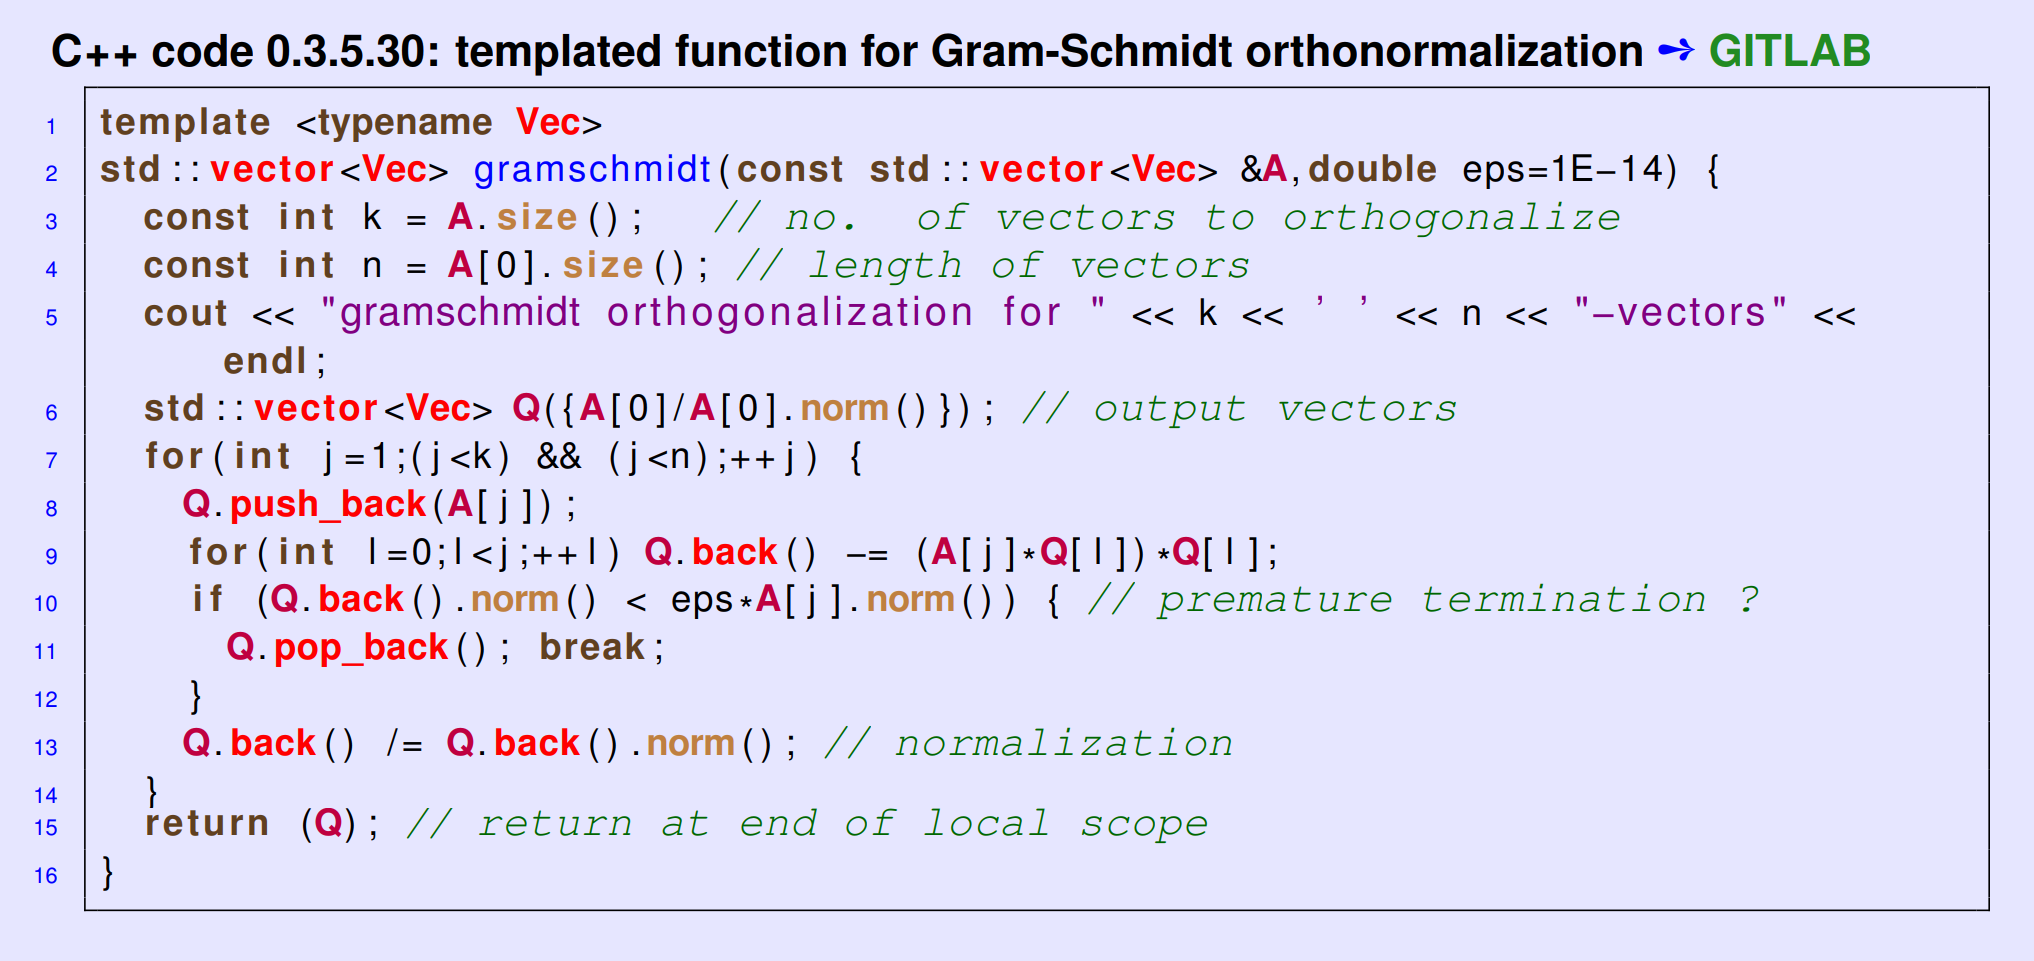
\includegraphics[width=1.0\linewidth]{GramSchmidtCode.png}
\end{figure}
\subsection*{1-2.a}
We are tasked with analysing the asymptotic complexity of the given function \verb|gramschmidt()| in terms of the matrix dimension $n$, if the argument \verb|A| has size $n \times n$ and it does not terminate prematurely $\\[1mm]$
The last part is important as it allows us to assume the worst case. We store the initial vector in $\mathbf{Q}$ in $\mathcal{O}\left(n\right)$, We can assume that the if statement is never executed as no premature termination occurs. If $\mathbf{A}$ is a $n \times n$ matrix, then we can see that $k$ and $n$ are equal, hence the outer loop simplifies to
\begin{lstlisting}
for(int j = 1; j < n; ++j) {
    ...
    for(int l = 0; l < j; ++l) {
        Q.back() -= (A[j] * Q[l]) * Q[l]; //O(n)
    }
    ...
}  
\end{lstlisting}
The operation performed in the inner loop is an inner product which is in $\mathcal{O}\left(n\right)$, we hence get $\mathcal{O}\left(n^{3}\right)$ overall, as we execute the inner loop body exactly $\frac{n\left(n-1\right)}{2}$ times if no premature termination occurs.

\pagebreak

\paragraph{1-2.b} 
We are now tasked with implementing the same method using EIGEN functions. Just looking at the given code might not be as helpful as actually looking at the original pseudo-code. 
\begin{figure}[!hbt]
    \centering
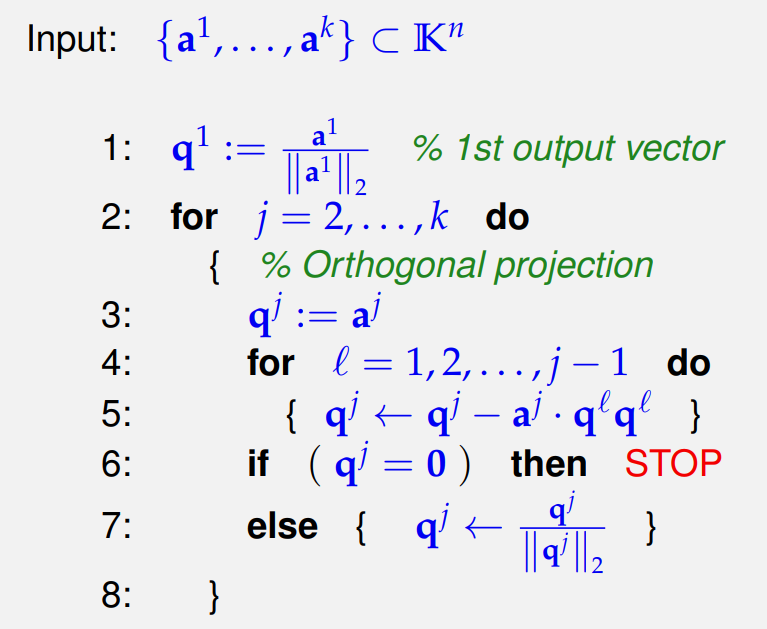
\includegraphics[width=0.4\linewidth]{GramSchmidtPseudoCode.png}
\end{figure}
\noindent Here we can see well how these operations could be vectorized, the inner loop does the following operation
\begin{equation*}
    q_{j} = q_{j} - \sum_{l=1}^{j-1} a_{j}\cdot q_{l} q_{l}
\end{equation*}
We can rewrite this as a block operation by computing $q_{j} =  q_{j} - Q_{1:j-1}\left(Q_{1:j-1}^{T} \cdot A_{j}\right) $ We can also use the fact that EIGEN has a built in function to normalize vectors given to us by \verb|normalize()|. This gives us the following code, in which we initialize $\mathbf{Q}$ with $\mathbf{A}$ as we always start with a column of $\mathbf{A}$ before calculating the orthogonalization. The usage of \verb|denorm| is not strictly needed, it is used because the \verb|norm| operation is not elementary and thus produces a different numerical error compared to base operations like addition and multiplication. Using a value like \verb|1E-9| works perfectly fine as well.
\begin{figure}[!hbt]
    \centering
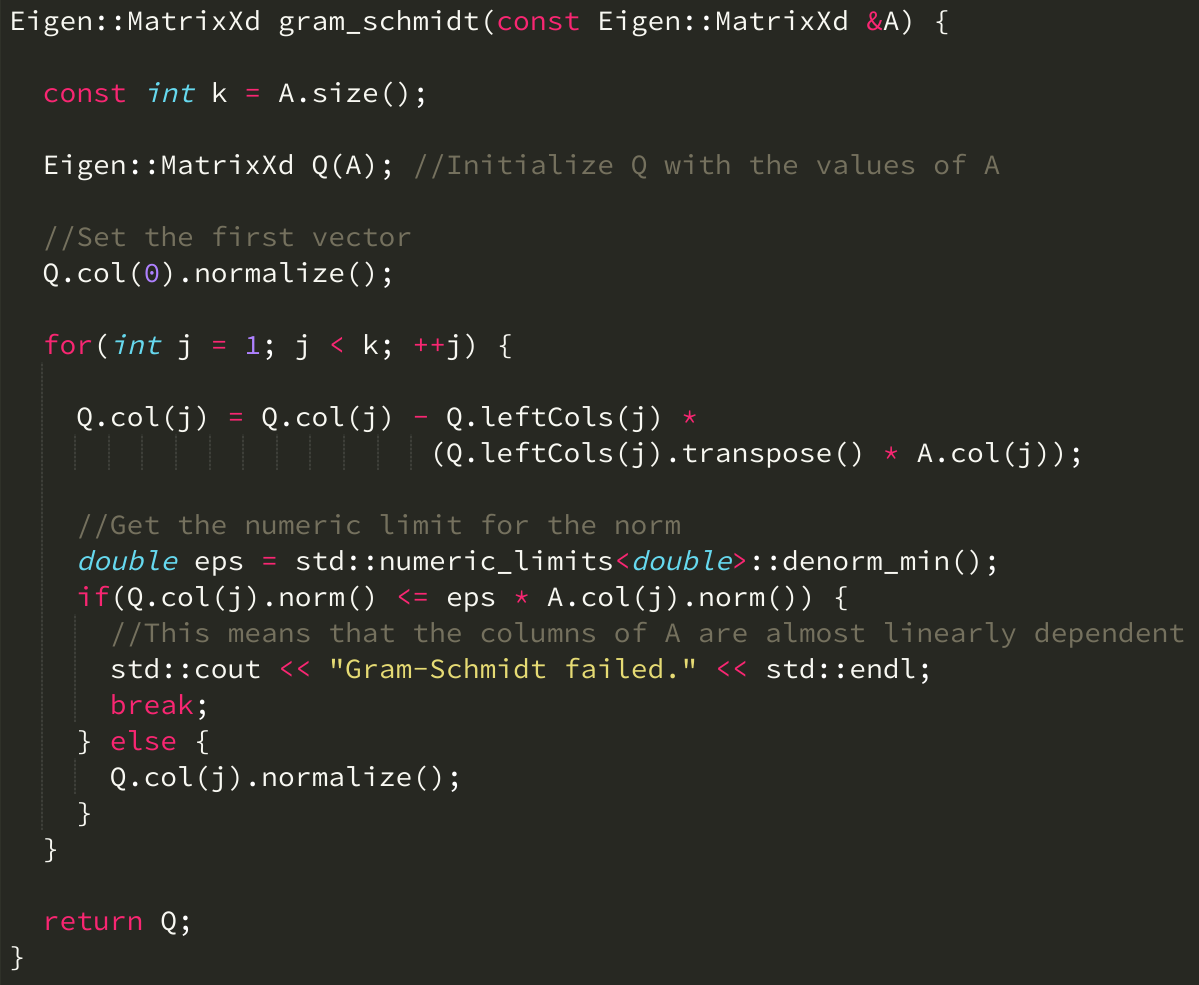
\includegraphics[width=0.7\linewidth]{1-2b.png}
\end{figure}

\pagebreak


\subsection*{1-2.c} We are now tasked with writing a method that tests our implementation for the matrix
\begin{equation*}
    \mathbf{A} \in \mathbb{R}^{n,n} \: , \: \left(VA\right)_{i,j} := i + 2j, \quad 1 \leq i, \, j \leq n
\end{equation*}
We remind ourselves that the matrix norm returned by Eigen when calling \verb|norm()| on a \verb|Eigen::MatrixXd| uses the Frobenius norm.
\begin{figure}[!hbt]
    \centering

\includegraphics[width=1.0\linewidth]{FrobeniusNorm.png}
\end{figure}
We now want to check if the result of our method (the matrix $\mathbf{Q}$) is orthonormal, i.e.
\begin{equation*}
    \mathbf{Q}\mathbf{Q}^{T} = \mathbf{Q}^{T}\mathbf{Q} = \mathbf{I}
\end{equation*}
The first hint then adives us to compare the norm against zero, which only makes sense if we we have
\begin{equation*}
    \left\lVert \mathbf{Q}^{T}\mathbf{Q} - \mathbf{I}\right\rVert_{F} \overset{!}{=} 0
\end{equation*}
We can however not check equality as results of numerical computations are almost always polluted by roundoff error (Remark 1.5.3.15). We should instead test against a relative error. We again use 
\begin{lstlisting}
    std::numeric_limits<double>::denorm_min();
\end{lstlisting}
\begin{figure}[!hbt]
    \centering
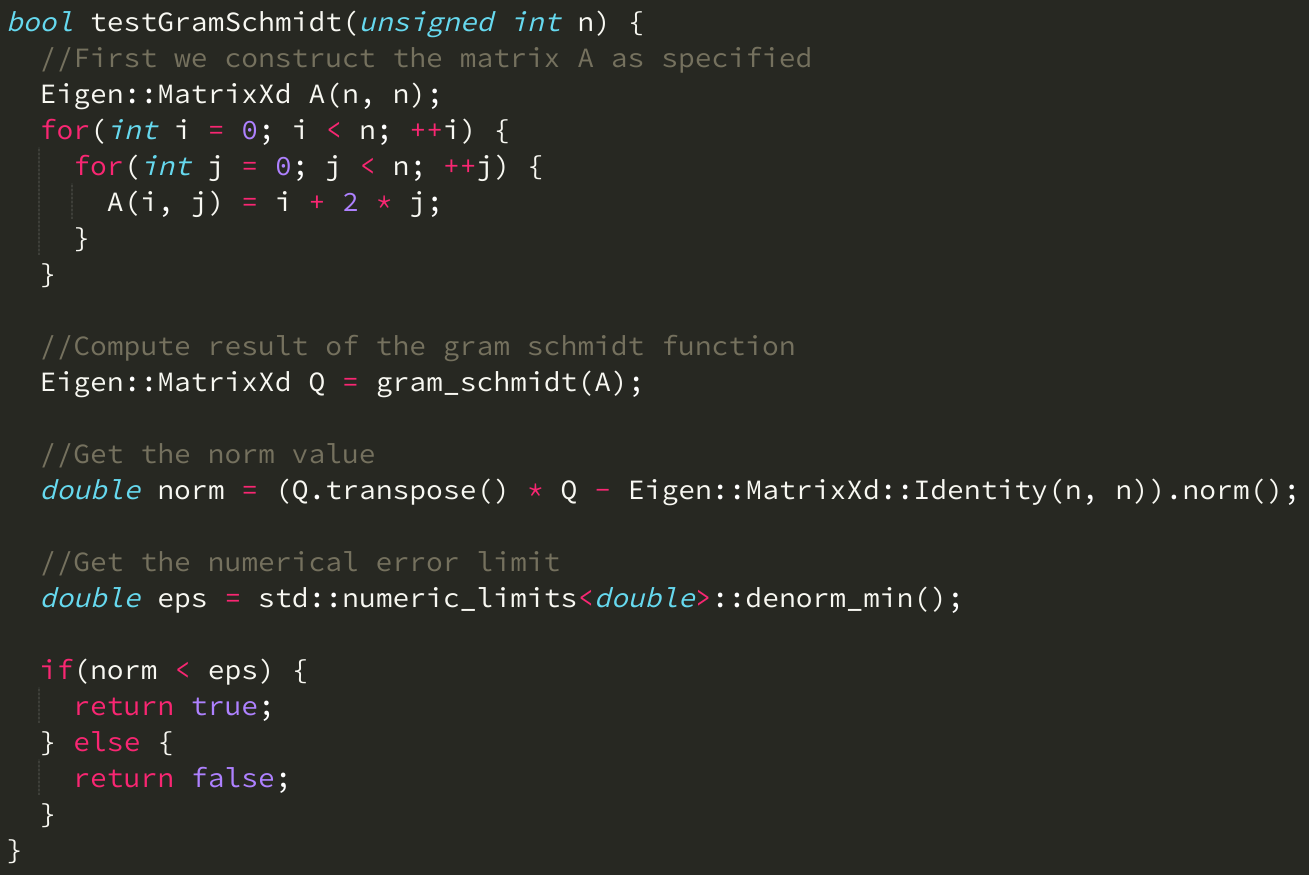
\includegraphics[width=0.9\linewidth]{1.2c.png}
\end{figure}
\end{document}
